\documentclass[11pt,a4paper]{article}
\usepackage{gtu-el-yazisi}
\begin{document}
\notbilgi{Analog Haberleşme}{Fourier serisi, Fourier dönüşümü ve özellikleri}{Ders4.pdf}

\sayfa{1}
\elcizimi[0.7]{sekiller/Ders4-s1-1.png}[1]

\begin{align*}
x(t)&=\frac12+\frac{2}{\pi}\Bigl[\cos(\omega_0 t)-\frac13\cos(3\omega_0 t)+\frac15\cos(5\omega_0 t)-\frac17\cos(7\omega_0 t)+\cdots\Bigr]\\
x_n(t)&=2x(t)-1=\frac{4}{\pi}\Bigl[\ \downarrow\ \Bigr]
\end{align*}

\begin{align*}
x(t)&=\sum_{n=-\infty}^{+\infty} x_n\, e^{jn\omega_0 t}\\
x_n&=\frac{1}{T_0}\int_{T_0} x(t)\,e^{-jn\omega_0 t}\,dt\\
P_x&=\sum_{n=-\infty}^{+\infty}|x_n|^2
\end{align*}

\begin{ornek}
$x(t)=2\sin(100t)$ işaretinin gücünü bulunuz
\end{ornek}

\[
\omega_0=100=\frac{2\pi}{T_0}\ \to\ T_0=\frac{2\pi}{\omega_0}=\frac{2\pi}{100}=\frac{\pi}{50}
\]

\[
P_x=\frac{1}{T_0}\int_{T_0}|x(t)|^2\,dt=\frac{1}{\pi/50}\int_{-\pi/100}^{\pi/100}4\underbrace{\sin^2(100t)}_{\frac12[1-\cos(200t)]}\,dt=\frac{100}{\pi}\Bigl[t-\frac{\sin(200t)}{200}\Bigr]_{-\pi/100}^{\pi/100}
\]

\[
=\frac{100}{\pi}\Bigl\{\Bigl[\frac{\pi}{100}-\frac{\sin\bigl(200\cdot\frac{\pi}{100}\bigr)}{200}\Bigr]-\Bigl[-\frac{\pi}{100}-\frac{\sin\bigl(200\cdot\frac{-\pi}{100}\bigr)}{200}\Bigr]\Bigr\}
\]

\[
=\frac{100}{\pi}\cdot\frac{2\pi}{100}=2\,\mathrm{Watt}
\]

\[
P_x=\frac{A^2}{2}=\frac{2^2}{2}=2\,\mathrm{Watt}\;/\!/
\]

\[
x(t)=2\sin(100t)=2\,\frac{e^{j100t}-e^{-j100t}}{2j}=\underbrace{\frac1j}_{x_1}e^{j100t}\ \underbrace{-\frac1j}_{x_{-1}}e^{-j100t}
\]

\[
P_x=\sum_n|x_n|^2=\Bigl|\frac1j\Bigr|^2+\Bigl|-\frac1j\Bigr|^2=1+1=2\,\mathrm{watt}
\]

\[ \star\ \ \sin\alpha=\frac{e^{j\alpha}-e^{-j\alpha}}{2j}\qquad\qquad \cos\alpha=\frac{e^{j\alpha}+e^{-j\alpha}}{2} \]

\sayfa{2}
\section{Fourier Dönüşümü}
\begin{itemize}
\item Periyodik olmayan işaretler için
\item Dirichlet şartları (T$_0$ yerine belirli aralıkta ifadesi \okunamadi{g.})
\end{itemize}

\begin{align*}
X(f)&=\Fou{x(t)}=\int_{-\infty}^{+\infty}x(t)\,e^{-j2\pi ft}\,dt\\
x(t)&=\iFou{X(f)}=\int_{-\infty}^{\infty}X(f)\cdot e^{j2\pi ft}\,df
\end{align*}

\[
x(t)\overset{F}{\longleftrightarrow}X(f)\ \Rightarrow\ X(f)=\underbrace{|X(f)|}_{\substack{\text{Genlik spektrumu}\\\text{(magnitude)}\\\uparrow\ \text{her zaman pozitif}}}e^{j\theta_x(f)}\ \text{\footnotesize$\searrow$ faz spektrumu}
\]

\begin{ornek}
$x(t)=\delta(t)$
\end{ornek}
\begin{align*}
X(f)&=\int_{-\infty}^{+\infty}\delta(t)\,e^{-j2\pi ft}\,dt\\
&=e^{-j2\pi f\cdot 0}=1
\end{align*}
\formulkutu[önemli]{\star\ \delta(t)\overset{F}{\longleftrightarrow}1}

\begin{ornek}
$X(f)=\delta(f)$
\end{ornek}
\[
x(t)=\int_{-\infty}^{\infty}\delta(f)\,e^{j2\pi ft}\,df=e^{j2\pi\cdot 0\cdot t}=1
\]
\formulkutu[önemli]{1\overset{F}{\longleftrightarrow}\delta(f)}

\begin{ornek}
$x(t)=A\,\Pi\!\left(\dfrac{t}{\tau}\right)$
\end{ornek}
\begin{center}
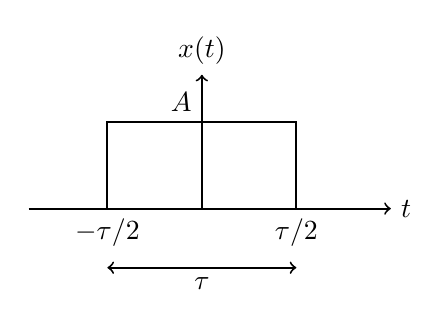
\begin{tikzpicture}[line width=0.7pt]
  \draw[->] (-2.2,0) -- (2.4,0) node[right] {$t$};
  \draw[->] (0,0) -- (0,1.7) node[above] {$x(t)$};
  \draw (-1.2,0) -- (-1.2,1.1) -- (1.2,1.1) -- (1.2,0);
  \node[above left] at (0,1.1) {$A$};
  \node[below] at (-1.2,0) {$-\tau/2$};
  \node[below] at (1.2,0) {$\tau/2$};
  \draw[<->] (-1.2,-0.75) -- (1.2,-0.75) node[midway,below] {$\tau$};
\end{tikzpicture}
\end{center}
\begin{align*}
X(f)&=\int_{-\tau/2}^{\tau/2}A\,e^{-j2\pi ft}\,dt\\
&=A\,\frac{e^{-j2\pi ft}}{-j2\pi f}\Bigg|_{-\tau/2}^{\tau/2}=A\Bigl[\frac{e^{-j2\pi f\tau/2}-e^{j2\pi f\tau/2}}{-j2\pi f}\Bigr]=\\
X(f)&=\frac{A}{\pi f\,\textcolor{kirmizikalem}{\cdot\tau}}\sin(\pi f\tau)\,\textcolor{kirmizikalem}{\cdot\tau}\\
X(f)&=A\tau\,\mathrm{sinc}(f\tau)
\end{align*}
\formulkutu[önemli]{x(t)=A\,\Pi\!\left(\frac{t}{\tau}\right)\overset{F}{\longleftrightarrow}X(f)=A\tau\,\mathrm{sinc}(f\tau)}

\sayfa{3}
\begin{center}
\begin{tikzpicture}[line width=0.7pt, x=0.95cm, y=1cm]
  \draw[->] (-6.6,0) -- (6.1,0) node[right] {$f$};
  \draw[->] (0,-0.55) -- (0,2.3) node[above] {$X(f)$};
  \draw[domain=-6.3:5.7,samples=400,smooth,variable=\x] plot ({\x},{2*sin(180*\x)/(pi*\x)});
  \node[right,text=kirmizikalem] at (0.05,2.05) {$A\tau$};
  \foreach \k in {-6,-5,-4,-3,-2,-1,1,2,3,4,5} {
    \draw (\k,0.06) -- (\k,-0.06);
    \node[below,font=\scriptsize] at (\k,-0.06) {$\frac{\k}{\tau}$};
  }
\end{tikzpicture}
\end{center}

\[
f\tau=k,\quad k\in\mathbb{Z}-\{0\}\ \Rightarrow\ \mathrm{sinc}(k)=0
\]
\[
f=\frac{k}{\tau}
\]

\section{Band Genişliği (BG) (Bandwidth-BW)}
Temel band \textcolor{kirmizikalem}{(bileşenler 0 Hz'in civarında)} işaretleri için genlik spektrumun sıfırdan farklı olduğu en yüksek pozitif frekansa BG denir.

\begin{center}
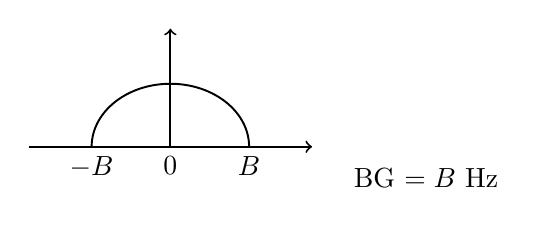
\begin{tikzpicture}[line width=0.7pt]
  \draw[->] (-1.8,0) -- (1.8,0);
  \draw[->] (0,0) -- (0,1.5);
  \draw (-1,0) arc[start angle=180,end angle=0,x radius=1,y radius=0.8];
  \node[below] at (-1,0) {$-B$};
  \node[below] at (0,0) {$0$};
  \node[below] at (1,0) {$B$};
  \node[right] at (2.2,-0.4) {BG $=B$ Hz};
\end{tikzpicture}
\end{center}

\textcolor{kirmizikalem}{Band geçiren (Bandpass)} işaretler için genlik spektrumun sıfırdan farklı olduğu pozitif frekanslar bölgesinin genişliğine BG denir.

\begin{center}
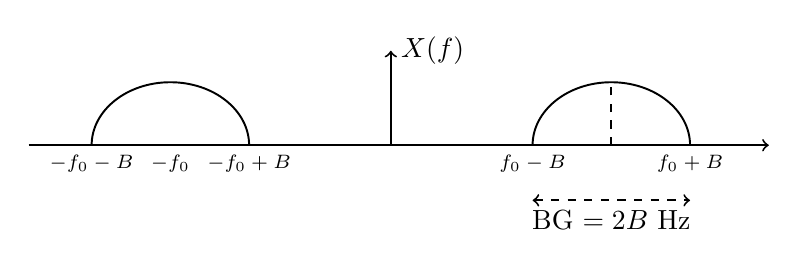
\begin{tikzpicture}[line width=0.7pt]
  \draw[->] (-4.6,0) -- (4.8,0);
  \draw[->] (0,0) -- (0,1.2) node[right] {$X(f)$};
  \draw (-3.8,0) arc[start angle=180,end angle=0,x radius=1,y radius=0.8];
  \draw (1.8,0) arc[start angle=180,end angle=0,x radius=1,y radius=0.8];
  \draw[dashed] (2.8,0) -- (2.8,0.8);
  \node[below,font=\scriptsize] at (-3.8,0) {$-f_0-B$};
  \node[below,font=\scriptsize] at (-2.8,0) {$-f_0$};
  \node[below,font=\scriptsize] at (-1.8,0) {$-f_0+B$};
  \node[below,font=\scriptsize] at (1.8,0) {$f_0-B$};
  \node[below,font=\scriptsize] at (3.8,0) {$f_0+B$};
  \draw[dashed,<->] (1.8,-0.7) -- (3.8,-0.7);
  \node[below] at (2.8,-0.7) {BG $=2B$ Hz};
\end{tikzpicture}
\end{center}

Sinc'in teorik olarak BG$=\infty$

\textcolor{kirmizikalem}{\%90 BG $=$ effective bant genişliği $=$ BG $=1/\tau$}

\noindent
\begin{minipage}[c]{0.4\linewidth}
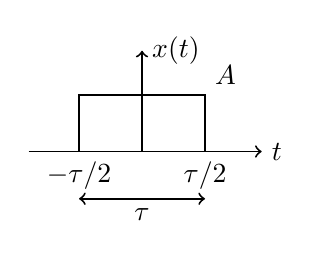
\begin{tikzpicture}[line width=0.7pt, scale=0.8]
  \draw[->] (-1.8,0) -- (1.9,0) node[right] {$t$};
  \draw[->] (0,0) -- (0,1.6) node[right] {$x(t)$};
  \draw (-1,0) -- (-1,0.9) -- (1,0.9) -- (1,0);
  \node[above right] at (1,0.9) {$A$};
  \node[below] at (-1,0) {$-\tau/2$};
  \node[below] at (1,0) {$\tau/2$};
  \draw[<->] (-1,-0.75) -- (1,-0.75) node[midway,below] {$\tau$};
\end{tikzpicture}
\end{minipage}
\hfill
\begin{minipage}[c]{0.55\linewidth}
\centering
\begin{tabular}{ccc}
Genişlik & & BG \\
{\footnotesize (zaman domeninde)} & & {\footnotesize (frekans domeninde)} \\
$\tau$ & $\times$ & BG $=1/\tau$
\end{tabular}
\end{minipage}

Veri hızıyla bant genişliği arasında doğrudan ilişki var.

{\small FTM}

\sayfa{4}
\section{Lineerlik özelliği}
\begin{align*}
x_1(t)&\overset{F}{\longleftrightarrow}X_1(f)\\
x_2(t)&\overset{F}{\longleftrightarrow}X_2(f)
\end{align*}
$a,b$ sabit
\[
x_3(t)=a\,x_1(t)+b\,x_2(t)\overset{F}{\longleftrightarrow}a\,X_1(f)+b\,X_2(f)=X_3(f)
\]

\section{Dualite (Simetri) özelliği}
\begin{align*}
x(t)&\overset{F}{\longleftrightarrow}X(f)\\
X(t)&\overset{F}{\longleftrightarrow}x(-f)
\end{align*}

\begin{center}
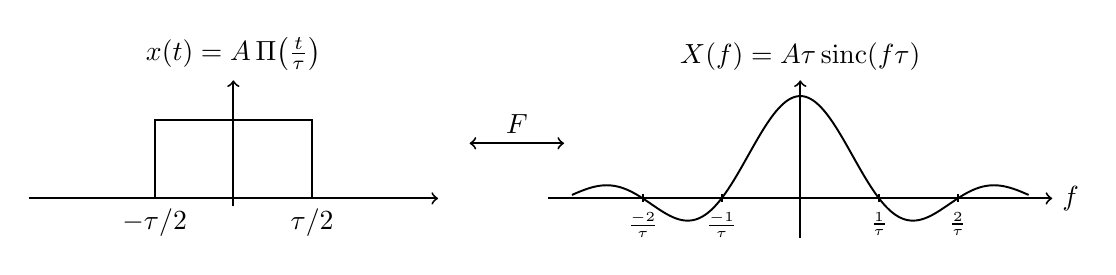
\begin{tikzpicture}[line width=0.7pt]
  \draw[->] (-2.6,0) -- (2.6,0);
  \draw[->] (0,-0.1) -- (0,1.5) node[above] {$x(t)=A\,\Pi\!\left(\frac{t}{\tau}\right)$};
  \draw (-1,0) -- (-1,1.0) -- (1,1.0) -- (1,0);
  \node[below] at (-1,0) {$-\tau/2$};
  \node[below] at (1,0) {$\tau/2$};
  \draw[<->] (3.0,0.7) -- (4.2,0.7) node[midway,above] {$F$};
  \begin{scope}[xshift=7.2cm,x=1.0cm,y=1cm]
    \draw[->] (-3.2,0) -- (3.2,0) node[right] {$f$};
    \draw[->] (0,-0.5) -- (0,1.5) node[above] {$X(f)=A\tau\,\mathrm{sinc}(f\tau)$};
    \draw[domain=-2.9:2.9,samples=200,smooth,variable=\x] plot ({\x},{1.3*sin(180*\x)/(pi*\x)});
    \foreach \k in {-2,-1,1,2} {\draw (\k,0.05) -- (\k,-0.05); \node[below,font=\scriptsize] at (\k,-0.05) {$\frac{\k}{\tau}$};}
  \end{scope}
\end{tikzpicture}
\end{center}

\[
X(t)=A\tau\,\mathrm{sinc}(t\tau)\overset{F}{\longleftrightarrow}x(-f)=A\,\Pi\!\left(\frac{-f}{\tau}\right)=A\,\Pi\!\left(\frac{f}{\tau}\right)
\]

\begin{center}
\begin{tikzpicture}[line width=0.7pt]
  \begin{scope}[x=1.0cm,y=1cm]
    \draw[->] (-3.2,0) -- (3.2,0) node[right,text=kirmizikalem] {$t$};
    \draw[->] (0,-0.5) -- (0,1.7) node[above] {$X(t)$};
    \draw[domain=-2.9:2.9,samples=200,smooth,variable=\x] plot ({\x},{1.5*sin(180*\x)/(pi*\x)});
    \foreach \k in {-2,-1,1,2} {\draw (\k,0.05) -- (\k,-0.05); \node[below,font=\scriptsize] at (\k,-0.05) {$\frac{\k}{\tau}$};}
  \end{scope}
  \begin{scope}[xshift=7.4cm]
    \draw[->] (-2.4,0) -- (2.6,0) node[right] {$f$};
    \draw[->] (0,0) -- (0,1.5);
    \draw (-1,0) -- (-1,0.9) -- (1,0.9) -- (1,0);
    \node[above right] at (0,0.9) {$A$};
    \node[below] at (-1,0) {$-\tau/2$};
    \node[below] at (1,0) {$\tau/2$};
  \end{scope}
\end{tikzpicture}
\end{center}

\[
A\tau\,\mathrm{sinc}(t\tau)\overset{F}{\longleftrightarrow}A\,\Pi\!\left(\frac{f}{\tau}\right)
\]

\section{Zamanda öteleme özelliği (Time shifting property)}
\begin{align*}
x(t)&\overset{F}{\longleftrightarrow}X(f)\\
x(t-t_0)&\overset{F}{\longleftrightarrow}X(f)\cdot e^{-j2\pi ft_0}
\end{align*}

\textcolor{kirmizikalem}{İspat:}
\[
\Fou{x(t-t_0)}=\int_{-\infty}^{\infty}x(t-t_0)\,e^{-j2\pi ft}\,dt
\]
\[
\begin{aligned}t-t_0&=t'\ \Rightarrow\ t=t_0+t'\\dt&=dt'\end{aligned}
\]
\[
=\int_{-\infty}^{+\infty}x(t')\,\underbrace{e^{-j2\pi f(t_0+t')}}_{e^{-j2\pi ft_0}\cdot e^{-j2\pi ft'}}\,dt'
\]

\sayfa{5}
\[
=e^{-j2\pi ft_0}\underbrace{\int_{-\infty}^{\infty}x(t')\,e^{-j2\pi ft'}\,dt'}_{X(f)}
\]

\section{Frekansta öteleme özelliği}
\begin{align*}
x(t)&\overset{F}{\longleftrightarrow}X(f)\\
x(t)\cdot e^{j2\pi f_0t}&\overset{F}{\longleftrightarrow}X(f-f_0)
\end{align*}
$f_0=$ sabit

\textcolor{kirmizikalem}{İspat:}
\begin{align*}
\Fou{x(t)\,e^{j2\pi f_0t}}&=\int_{-\infty}^{\infty}x(t)\,\underbrace{e^{j2\pi f_0t}\cdot e^{-j2\pi ft}}_{e^{-j2\pi(f-f_0)t}}\,dt\\
&=\int_{-\infty}^{\infty}x(t)\,e^{-j2\pi\underbrace{(f-f_0)}_{f'}t}\,dt\\
&=X(f')=X(f-f_0)
\end{align*}

\begin{ornek}
\begin{center}
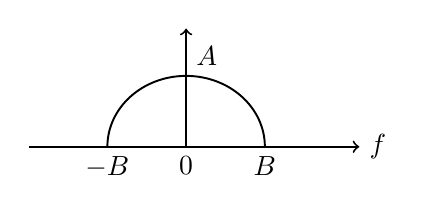
\begin{tikzpicture}[line width=0.7pt]
  \draw[->] (-2,0) -- (2.2,0) node[right] {$f$};
  \draw[->] (0,0) -- (0,1.5);
  \draw (-1,0) arc[start angle=180,end angle=0,x radius=1,y radius=0.9];
  \node[above right] at (0,0.9) {$A$};
  \node[below] at (-1,0) {$-B$};
  \node[below] at (0,0) {$0$};
  \node[below] at (1,0) {$B$};
\end{tikzpicture}
\qquad
$\Fou{x(t)\cdot e^{j2\pi f_0t}}=X(f-f_0)$

\bigskip
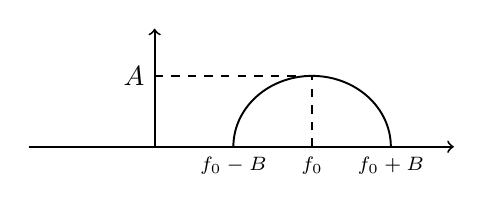
\begin{tikzpicture}[line width=0.7pt]
  \draw[->] (-1.6,0) -- (3.8,0);
  \draw[->] (0,0) -- (0,1.5);
  \draw (1,0) arc[start angle=180,end angle=0,x radius=1,y radius=0.9];
  \draw[dashed] (2,0) -- (2,0.9);
  \draw[dashed] (0,0.9) -- (2,0.9);
  \node[left] at (0,0.9) {$A$};
  \node[below,font=\scriptsize] at (1,0) {$f_0-B$};
  \node[below,font=\scriptsize] at (2,0) {$f_0$};
  \node[below,font=\scriptsize] at (3,0) {$f_0+B$};
\end{tikzpicture}
\end{center}
\end{ornek}

\begin{ornek}
$x(t)=\cos(2\pi f_0t)=\dfrac12\left[e^{j2\pi f_0t}+e^{-j2\pi f_0t}\right]$
\end{ornek}
\begin{align*}
1&\longleftrightarrow\delta(f)\\
x(t)\,e^{j2\pi f_0t}&\overset{F}{\longleftrightarrow}X(f-f_0)
\end{align*}
\[
1\cdot e^{j2\pi f_0t}\overset{F}{\longleftrightarrow}\delta(f-f_0)\ \longrightarrow\ 
\begin{array}{c}x(t)=\cos(2\pi f_0t)\\ \Big\updownarrow F\\ X(f)=\tfrac12\bigl[\delta(f-f_0)+\delta(f+f_0)\bigr]\end{array}
\]

\formulkutu[önemli]{\cos(2\pi f_0t)\overset{F}{\longleftrightarrow}\tfrac12\bigl[\delta(f-f_0)+\delta(f+f_0)\bigr]}

\begin{align*}
X(f)&=|X(f)|\\
\theta_x(f)&=0
\end{align*}
\begin{center}
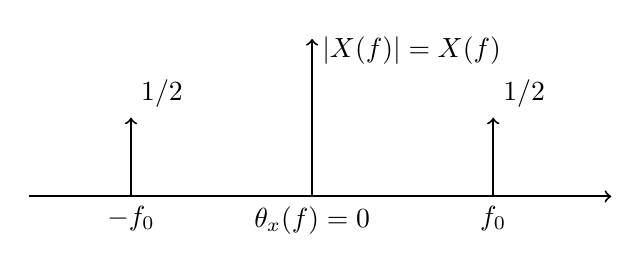
\begin{tikzpicture}[line width=0.7pt]
  \draw[->] (-3.6,0) -- (3.8,0);
  \draw[->] (0,0) -- (0,2.0);
  \node[right] at (0,1.85) {$|X(f)|=X(f)$};
  \draw[->] (-2.3,0) -- (-2.3,1.0);
  \node[above right] at (-2.3,1.0) {$1/2$};
  \draw[->] (2.3,0) -- (2.3,1.0);
  \node[above right] at (2.3,1.0) {$1/2$};
  \node[below] at (-2.3,0) {$-f_0$};
  \node[below] at (2.3,0) {$f_0$};
  \node[below] at (0,0) {$\theta_x(f)=0$};
\end{tikzpicture}
\end{center}

\sayfa{6}
\begin{align*}
x(t)&=\sin(2\pi f_0t)=\frac{1}{2j}\left[e^{j2\pi f_0t}-e^{-j2\pi f_0t}\right]\\
X(f)&=\frac{1}{2j}\bigl[\delta(f-f_0)-\delta(f+f_0)\bigr]
\end{align*}
\[
j=e^{j\pi/2}
\]
\textcolor{kirmizikalem}{$e^{\pm j\alpha}=\cos\alpha\pm j\sin\alpha$}
\[
X(f)=\frac12\bigl[\delta(f-f_0)\,e^{-j\pi/2}+\delta(f+f_0)\,e^{j\pi/2}\bigr]
\]

\begin{center}
\begin{tikzpicture}[line width=0.7pt]
  \draw[->] (-3.2,0) -- (3.6,0) node[right] {$f$};
  \draw[->] (0,0) -- (0,1.8) node[above] {$|X(f)|$};
  \draw[->] (-1.9,0) -- (-1.9,0.9);
  \node[above right] at (-1.9,0.9) {$1/2$};
  \draw[->] (1.6,0) -- (1.6,0.9);
  \node[above right] at (1.6,0.9) {$1/2$};
  \node[below] at (-1.9,0) {$-f_0$};
  \node[below] at (1.6,0) {$f_0$};
\end{tikzpicture}
\end{center}
\begin{center}
\begin{tikzpicture}[line width=0.7pt]
  \draw[->] (-2.6,0) -- (3.6,0) node[right] {$f$};
  \draw[->] (0,-1.1) -- (0,1.3) node[above right] {$\theta_x(f)$};
  \fill (-1.4,0.9) circle (1.5pt);
  \draw[dashed] (-1.4,0) -- (-1.4,0.9) -- (0,0.9);
  \node[right,font=\scriptsize] at (0,0.9) {$\pi/2$};
  \draw (1.4,0) -- (1.4,-0.9);
  \draw[dashed] (0,-0.9) -- (1.4,-0.9);
  \node[left,font=\scriptsize] at (0,-0.9) {$-\pi/2$};
  \node[below] at (-1.4,0) {$-f_0$};
  \node[above] at (1.4,0) {$f_0$};
\end{tikzpicture}
\end{center}

\section{Modülasyon özelliği}
\begin{align*}
x(t)&\overset{F}{\longleftrightarrow}X(f)\\
\underbrace{y(t)}_{\textcolor{kirmizikalem}{\text{modüle edilmiş işaret}}}&=\underbrace{x(t)}_{\textcolor{kirmizikalem}{\text{mesaj işareti}}}\cdot\overbrace{\underbrace{\cos(2\pi f_0t)}_{\frac12\left[e^{j2\pi f_0t}+e^{-j2\pi f_0t}\right]}}^{\textcolor{kirmizikalem}{\text{taşıyıcı işaret (Carrier Signal)}}}\\
&\overset{F}{\longleftrightarrow}Y(f)=\frac12\bigl[X(f-f_0)+X(f+f_0)\bigr]
\end{align*}

\begin{center}
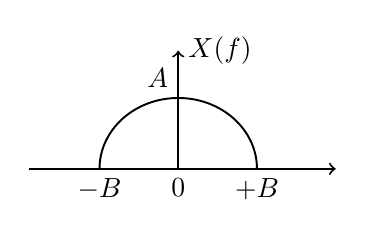
\begin{tikzpicture}[line width=0.7pt]
  \draw[->] (-1.9,0) -- (2.0,0);
  \draw[->] (0,0) -- (0,1.5) node[right] {$X(f)$};
  \draw (-1,0) arc[start angle=180,end angle=0,x radius=1,y radius=0.9];
  \node[above left] at (0,0.9) {$A$};
  \node[below] at (-1,0) {$-B$};
  \node[below] at (0,0) {$0$};
  \node[below] at (1,0) {$+B$};
\end{tikzpicture}
\end{center}
\begin{center}
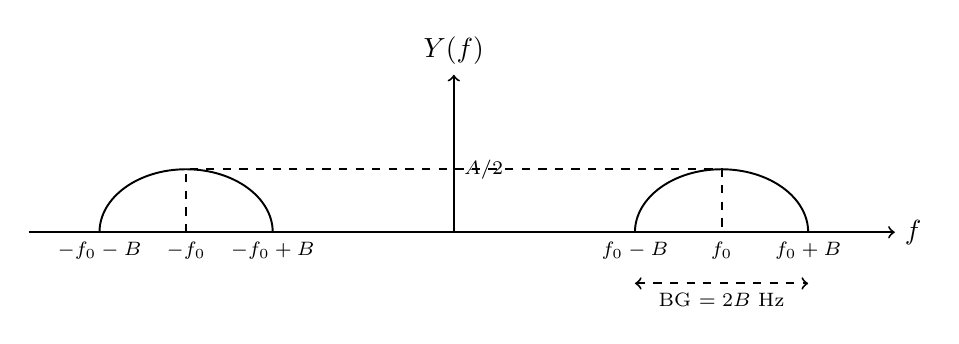
\begin{tikzpicture}[line width=0.7pt]
  \draw[->] (-5.4,0) -- (5.6,0) node[right] {$f$};
  \draw[->] (0,0) -- (0,2.0) node[above] {$Y(f)$};
  \draw (-4.5,0) arc[start angle=180,end angle=0,x radius=1.1,y radius=0.8];
  \draw (2.3,0) arc[start angle=180,end angle=0,x radius=1.1,y radius=0.8];
  \draw[dashed] (-3.4,0) -- (-3.4,0.8) -- (3.4,0.8) -- (3.4,0);
  \node[right,font=\scriptsize] at (0,0.8) {$A/2$};
  \node[below,font=\scriptsize] at (-4.5,0) {$-f_0-B$};
  \node[below,font=\scriptsize] at (-3.4,0) {$-f_0$};
  \node[below,font=\scriptsize] at (-2.3,0) {$-f_0+B$};
  \node[below,font=\scriptsize] at (2.3,0) {$f_0-B$};
  \node[below,font=\scriptsize] at (3.4,0) {$f_0$};
  \node[below,font=\scriptsize] at (4.5,0) {$f_0+B$};
  \draw[dashed,<->] (2.3,-0.65) -- (4.5,-0.65);
  \node[below,font=\scriptsize] at (3.4,-0.65) {BG $=2B$ Hz};
\end{tikzpicture}
\end{center}

\textcolor{kirmizikalem}{frekans bölmeli çoklama}

\section{Ölçekleme özelliği (Scaling property)}
\begin{align*}
x(t)&\overset{F}{\longleftrightarrow}X(f)\\
x(at)&\overset{F}{\longleftrightarrow}\frac{1}{|a|}X\!\left(\frac{f}{a}\right)
\end{align*}
\[
a=2:\quad \underbrace{x(2t)}_{\textcolor{kirmizikalem}{\text{zamanda daralması}}}\longleftrightarrow\frac12\underbrace{X\!\left(\frac f2\right)}_{\textcolor{kirmizikalem}{\substack{\text{Frekansta}\\\text{genişlenir}}}}
\]

\textcolor{kirmizikalem}{İşaretin Genişliği $\times$ BG}

\sayfa{7}
\section{Konvülasyon özelliği}
\[
x(t)\circledast y(t)=\int_{-\infty}^{\infty}x(\tau)\,y(t-\tau)\,d\tau
\]
\begin{align*}
z(t)=x(t)\circledast y(t)&\overset{F}{\longleftrightarrow}Z(f)=X(f)\cdot Y(f)\\
z(t)=x(t)\cdot y(t)&\overset{F}{\longleftrightarrow}Z(f)=X(f)\circledast Y(f)
\end{align*}

\[
z(t)=\underbrace{x(t)}_{\textcolor{kirmizikalem}{\text{BG}=B_1}}\circledast\underbrace{y(t)}_{\textcolor{kirmizikalem}{\text{BG}=B_2}}\ \rightarrow\ \text{Genişlik}\{z(t)\}=\text{Genişlik}\{x(t)\}+\text{Genişlik}\{y(t)\}
\]
\[
z(t)=x(t)\cdot y(t)\ \Rightarrow\ Z(f)=\underbrace{X(f)}_{\text{BG}=B_1}\circledast\underbrace{Y(f)}_{\text{BG}=B_2}
\]
\[
\Big\downarrow\ \ \text{BG}=B_1+B_2
\]

\begin{ornek}
$\Lambda(t)=\Pi(t)\circledast\Pi(t)\ \Rightarrow\ \Fou{A\Lambda\!\left(\frac{t}{\tau}\right)}=\ ?$
\end{ornek}
\begin{align*}
\Fou{\Lambda(t)}&=\underbrace{\Fou{\Pi(t)}}_{\mathrm{sinc}\,f}\cdot\underbrace{\Fou{\Pi(t)}}_{\mathrm{sinc}\,f}=\mathrm{sinc}^2(f)\\
\Fou{A\Lambda\!\left(\tfrac{t}{\tau}\right)}&=A\tau\,\mathrm{sinc}^2(f\tau)
\end{align*}
\formulkutu[önemli]{A\Lambda\!\left(\tfrac{t}{\tau}\right)\overset{F}{\longleftrightarrow}A\tau\,\mathrm{sinc}^2(f\tau)}

\begin{center}
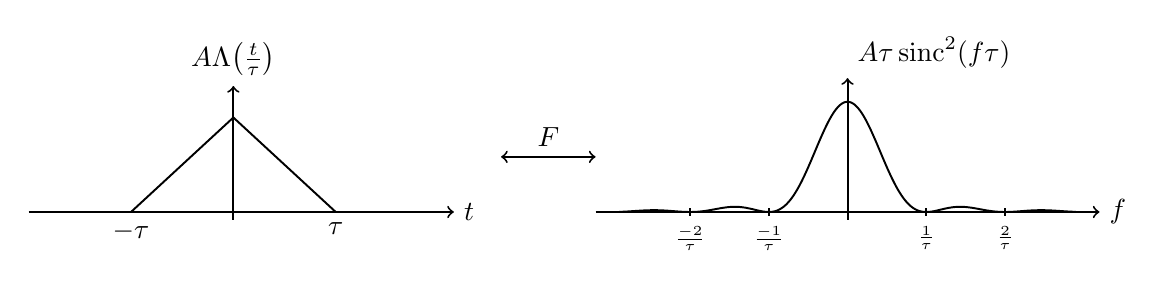
\begin{tikzpicture}[line width=0.7pt]
  \draw[->] (-2.6,0) -- (2.8,0) node[right] {$t$};
  \draw[->] (0,-0.1) -- (0,1.6) node[above] {$A\Lambda\!\left(\frac{t}{\tau}\right)$};
  \draw (-1.3,0) -- (0,1.2) -- (1.3,0);
  \node[below] at (-1.3,0) {$-\tau$};
  \node[below] at (1.3,0) {$\tau$};
  \draw[<->] (3.4,0.7) -- (4.6,0.7) node[midway,above] {$F$};
  \begin{scope}[xshift=7.8cm,x=1.0cm,y=1cm]
    \draw[->] (-3.2,0) -- (3.2,0) node[right] {$f$};
    \draw[->] (0,-0.1) -- (0,1.7) node[above right] {$A\tau\,\mathrm{sinc}^2(f\tau)$};
    \draw[domain=-2.9:2.9,samples=300,smooth,variable=\x] plot ({\x},{1.4*(sin(180*\x)/(pi*\x))^2});
    \foreach \k in {-2,-1,1,2} {\draw (\k,0.05) -- (\k,-0.05); \node[below,font=\scriptsize] at (\k,-0.05) {$\frac{\k}{\tau}$};}
  \end{scope}
\end{tikzpicture}
\end{center}

\sayfa{8}
\section{İntegral özelliği}
\begin{align*}
x(t)&\overset{F}{\longleftrightarrow}X(f)\\
y(t)=\int_{-\infty}^{t}x(\tau)\,d\tau&\overset{F}{\longleftrightarrow}Y(f)=\frac{X(f)}{j2\pi f}+\frac12\,\overbrace{X(0)}^{\textcolor{kirmizikalem}{\text{dc bileşeni}=X(f)|_{f=0}}}\delta(f)
\end{align*}
frekans arttıkça genliği azalıyor\\
(alçak geçiren filtre gibi davranıyor)

\begin{ornek}
$u(t)=\displaystyle\int_{-\infty}^{t}\delta(\tau)\,d\tau\overset{F}{\longleftrightarrow}\dfrac{1}{j2\pi f}+\dfrac12\cdot1\cdot\delta(f)$
\end{ornek}
\begin{align*}
u(t)&\overset{F}{\longleftrightarrow}\frac{1}{j2\pi f}+\frac12\delta(f)\\
\Fou{u(t)}&=\frac{1}{j2\pi f}+\frac12\delta(f)
\end{align*}
(bu $U(f)$ \okunamadi{eşit değeri})\\
$\hookrightarrow$ bu frekans uzayında birim basamak

\begin{ornek}
$\mathrm{Sgn}(t)=u(t)-\underbrace{u(-t)}_{\textcolor{kirmizikalem}{a=-1}}$
\end{ornek}
\begin{align*}
\Fou{\mathrm{sgn}(t)}&=\frac{1}{j2\pi f}+\frac12\delta(f)\\
&\quad-\frac{1}{|-1|}\left\{\frac{1}{j2\pi\frac{f}{-1}}+\frac12\underbrace{\delta\!\left(\frac{f}{-1}\right)}_{=\delta(f)}\right\}\\
&=\frac{1}{j\pi f}
\end{align*}
\formulkutu[önemli]{\mathrm{Sgn}(t)\overset{F}{\longleftrightarrow}\frac{1}{j\pi f}}

\section{Türev özelliği}
\begin{align*}
x(t)&\overset{F}{\longleftrightarrow}X(f)\\
y(t)=\frac{d}{dt}x(t)&\overset{F}{\longleftrightarrow}Y(f)=j2\pi f\,X(f)\quad\rightarrow\ \substack{\text{frekans arttıkça işaret}\\\text{güçlenir (yüksek geçiren f)}}\\
y(t)=\frac{d^n}{dt^n}x(t)&\overset{F}{\longleftrightarrow}Y(f)=(j2\pi f)^nX(f)
\end{align*}

\begin{ornek}
$x(t)=\Lambda\!\left(\dfrac{t}{\tau}\right)$'nun FD'nü türev özelliğini kullanarak bulunuz
\end{ornek}
\begin{center}
\begin{tikzpicture}[line width=0.7pt]
  \draw[->] (-2.4,0) -- (2.4,0);
  \draw[->] (0,-0.1) -- (0,1.7);
  \draw (-1.3,0) -- (0,1.2) -- (1.3,0);
  \node[left] at (0,1.2) {$1$};
  \node[below] at (-1.3,0) {$-\tau$};
  \node[below] at (1.3,0) {$\tau$};
  \node[left,font=\scriptsize,text=kirmizikalem] at (-0.65,0.6) {eğim $=1/\tau$};
  \node[right,font=\scriptsize,text=kirmizikalem] at (0.65,0.6) {eğim $=-1/\tau$};
\end{tikzpicture}
\end{center}

\sayfa{9}
\begin{center}
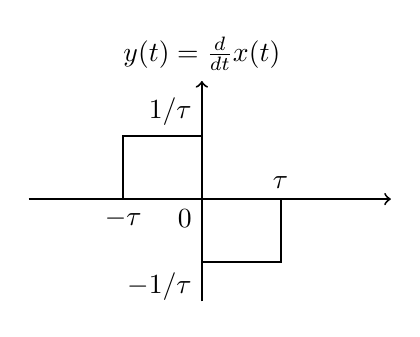
\begin{tikzpicture}[line width=0.7pt]
  \draw[->] (-2.2,0) -- (2.4,0);
  \draw[->] (0,-1.3) -- (0,1.5) node[above] {$y(t)=\frac{d}{dt}x(t)$};
  \draw (-1,0) -- (-1,0.8) -- (0,0.8);
  \draw (0,-0.8) -- (1,-0.8) -- (1,0);
  \node[above left] at (0,0.8) {$1/\tau$};
  \node[below] at (-1,0) {$-\tau$};
  \node[below left] at (0,0) {$0$};
  \node[above] at (1,0) {$\tau$};
  \node[below left] at (0,-0.8) {$-1/\tau$};
\end{tikzpicture}
\end{center}

\[
y(t)=\frac{d}{dt}x(t)
\]
\[
Y(f)=j2\pi f\,X(f)\ \rightarrow\ X(f)=\frac{Y(f)}{j2\pi f}
\]

\begin{center}
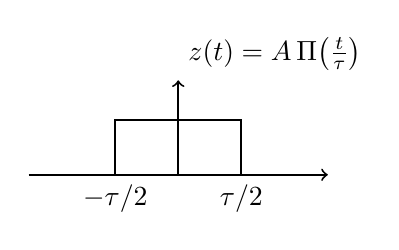
\begin{tikzpicture}[line width=0.7pt]
  \draw[->] (-1.9,0) -- (1.9,0);
  \draw[->] (0,0) -- (0,1.2) node[above right] {$z(t)=A\,\Pi\!\left(\frac{t}{\tau}\right)$};
  \draw (-0.8,0) -- (-0.8,0.7) -- (0.8,0.7) -- (0.8,0);
  \node[below] at (-0.8,0) {$-\tau/2$};
  \node[below] at (0.8,0) {$\tau/2$};
\end{tikzpicture}
\end{center}

\[
y(t)=z\!\left(t+\tfrac{\tau}{2}\right)-z\!\left(t-\tfrac{\tau}{2}\right)
\]
\begin{align*}
Y(f)&=Z(f)\,e^{j2\pi f\frac{\tau}{2}}-Z(f)\,e^{-j2\pi f\frac{\tau}{2}}\\
Y(f)&=Z(f)\left[e^{j\pi f\tau}-e^{-j\pi f\tau}\right]\\
X(f)&=\frac{Y(f)}{j2\pi f}=\frac{Z(f)}{j2\pi f}\left[e^{j\pi f\tau}-e^{-j\pi f\tau}\right]\\
&=\frac{Z(f)}{\pi f\,\textcolor{kirmizikalem}{\cdot\tau}}\,\sin(\pi f\tau)\,\textcolor{kirmizikalem}{\cdot\tau}
\end{align*}
\[
X(f)=\underbrace{Z(f)}_{\substack{\downarrow\\A\tau\,\mathrm{sinc}(f\tau)\\\downarrow\\1/\tau}}\cdot\,\tau\,\mathrm{sinc}(f\tau)=\tau\,\mathrm{sinc}^2(f\tau)
\]

\section{Periyodik işaretlerin FD}
$\forall t,\ x(t+T_0)=x(t)$

\formulkutu[önemli]{\begin{aligned}x(t)&=\sum_{n=-\infty}^{+\infty}x_n\,e^{jn\omega_0t}\\\omega_0&=2\pi f_0=\frac{2\pi}{T_0}\\x_n&=\frac{1}{T_0}\int_{T_0}x(t)\,e^{-jn\omega_0t}\,dt\end{aligned}}

\begin{align*}
e^{j2\pi f_0t}&\overset{F}{\longleftrightarrow}\delta(f-f_0)\\
e^{jn\omega_0t}=e^{jn2\pi f_0t}&\overset{F}{\longleftrightarrow}\delta(f-nf_0)
\end{align*}

\sayfa{10}
\[
x(t)=\sum_{n=-\infty}^{+\infty}x_n\,e^{j2\pi nf_0t}\overset{F}{\longleftrightarrow}X(f)=\sum_{n=-\infty}^{+\infty}x_n\,\delta(f-nf_0)
\]
cos ve sin fourier dönüşümü içeriyor onun için mantıklı.

\begin{ornek}
\begin{align*}
x(t)=\delta_{T_0}(t)&=\sum_{n=-\infty}^{+\infty}\delta(t-nT_0)=\frac{1}{T_0}\sum_{n=-\infty}^{+\infty}e^{j2\pi nf_0t}\\
&\overset{F}{\longleftrightarrow}X(f)=\frac{1}{T_0}\sum_{n=-\infty}^{\infty}\delta(f-nf_0)
\end{align*}
\end{ornek}
Dürtü katarı

\textcolor{kirmizikalem}{$\star$ t ve f'te dürtü katarı}

\begin{center}
\begin{tikzpicture}[line width=0.7pt]
  \draw[->] (-3.2,0) -- (3.0,0);
  \draw[->] (0,0) -- (0,1.9) node[above right] {$x(t)$};
  \foreach \k in {-2,-1,0,1,2} {\draw[->,kirmizikalem] (\k,0) -- (\k,1.0);}
  \node[above right,font=\scriptsize] at (0,1.0) {$1$};
  \node[below,font=\scriptsize] at (-2,0) {$-2T_0$};
  \node[below,font=\scriptsize] at (-1,0) {$-T_0$};
  \node[below,font=\scriptsize] at (0,0) {$0$};
  \node[below,font=\scriptsize] at (1,0) {$T_0$};
  \node[below,font=\scriptsize] at (2,0) {$2T_0$};
  \begin{scope}[xshift=7.6cm]
    \draw[->] (-3.2,0) -- (3.2,0) node[right] {$f$};
    \draw[->] (0,0) -- (0,1.9) node[above right] {$X(f)$};
    \foreach \k in {-2,-1,0,1,2} {\draw[->,kirmizikalem] (\k,0) -- (\k,1.0);}
    \node[right,font=\scriptsize] at (0.05,1.25) {$1/T_0=f_0$};
    \node[below,font=\scriptsize] at (-2,0) {$-2f_0$};
    \node[below,font=\scriptsize] at (-1,0) {$-f_0$};
    \node[below,font=\scriptsize] at (0,0) {$0$};
    \node[below,font=\scriptsize] at (1,0) {$f_0$};
    \node[below,font=\scriptsize] at (2,0) {$2f_0$};
  \end{scope}
\end{tikzpicture}
\end{center}

\section{Parseval Teoremi}
\[
\star\ \underbrace{E_x}_{\textcolor{kirmizikalem}{\text{Sınav sorusu}}}=\int_{-\infty}^{+\infty}|x(t)|^2\,dt=\int_{-\infty}^{\infty}\underbrace{|X(f)|^2}_{\text{Enerji yoğunluk fonksiyonu}}df
\]
\textcolor{kirmizikalem}{$\star\star$ $A\tau\,\mathrm{sinc}(t\tau)$ enerjisini bulunuz,\\ ama fourier dönüşümünden \okunamadi{yapsanız} -}

\[
\begin{array}{l}
x(t)\ \text{reel}\ \Rightarrow\ X(-f)=X^*(f)\\[6pt]
\star\ x(t)\ \text{reel ve çift}\ \Rightarrow\ X(f)\ \text{reel ve çift}\ \ \rightarrow\ X(-f)=X(f)\\[2pt]
\qquad\swarrow\ x^*(t)=x(t)\qquad\downarrow\ x(-t)=x(t)\qquad\hookrightarrow\ X^*(f)=X(f)\ \checkmark
\end{array}
\]
\textcolor{kirmizikalem}{$\star$ Ödev ispatla}

\[
\begin{array}{l}
x(t)\ \text{sanal ve tek ise}\ \Rightarrow\ X(f)\ \text{sanal ve tek}\\[2pt]
\qquad\qquad\downarrow\ X^*(f)=-X(f)\qquad\hookrightarrow\ X(-f)=-X(f)
\end{array}
\]

\end{document}
